\section{Proceso B\'asico del Reconocimiento del Habla}

\begin{frame}{Proceso B\'asico del Reconocimiento del Habla}
Para un lenguaje $L$ y una entrada ac\'ustica $X$, el problema del reconocimiento del habla puede 
definirse como \cite{Jurafsky}:

\begin{quote}
\emph{La b\'usqueda de la oraci\'on m\'as probable perteneciente al lenguaje L, dada la entrada ac\'ustica X.}
\end{quote}

Sean $O = o_1,o_2,\ldots,o_T$ la secuencia de $T$ observaciones ac\'usticas de entrada y 
$W  = w_1,w_2,\ldots,w_M$ la secuencia de $M$ palabras de salida. Siendo $\hat{W}$ una aproximaci\'on 
probabil{\'\i}stica de $W$, el enfoque estad{\'\i}stico define el problema de reconocimiento del habla 
mediante la ecuaci\'on (\ref{eq:asrFundamental}) \cite{Jurafsky}:

\begin{align}
\hat{W} = \argmax_{W \in L} \overbrace{P(O|W)}^\text{M. ac\'ustico}\overbrace{P(W)}^\text{M. de lenguaje}
\label{eq:asrFundamental}
\end{align}
\end{frame}

\begin{frame}{Proceso B\'asico del Reconocimiento del Habla (2)}
El proceso b\'asico del reconocimiento del habla, puede descomponerse en dos etapas o fases, 
cada una de las cuales recibe una entrada (o varias) y produce una salida determinada.

\begin{figure}[H] 
\centering
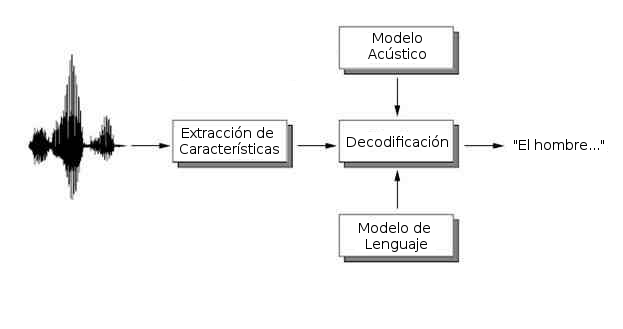
\includegraphics[width=0.8\textwidth]{./graphics/proceso.png}
\caption{Proceso del reconocimiento del habla. Traducido a partir de \protect\cite{VerenichASR}.}
\label{figure:proceso}
\end{figure}
\end{frame}


\begin{frame}{Proceso B\'asico del Reconocimiento del Habla (3)}
El modelo ac\'ustico y el modelo de lenguaje pueden requerir una fase de entrenamiento previa,
durante la cual se utilizan datos de entrenamiento (audio y texto) para estimar los valores adecuados 
para los par\'ametros de los modelos.
\end{frame}

\begin{frame}{Proceso B\'asico del Reconocimiento del Habla (4)}
\framesubtitle{Fase 1: Extracci\'on de caracter{\'\i}sticas}

La fase de extracci\'on de caracter{\'\i}sticas inicia con la recepci\'on de una onda sonora, correspondiente a la voz.
La misma puede caracterizarse mediante los formantes \cite{Fant1960acoustic} que se observan en un espectrograma.

Durante esta fase se sigue un proceso de an\'alisis de se\~nal: muestreo, cuantificaci\'on y conversi\'on.
Los detalles de este proceso dependen del conjunto de caracter{\'\i}sticas espectrales seleccionado 
para representar la se\~nal. Ejemplos de estos conjuntos son las caracter{\'\i}sticas basadas en codificaci\'on
predictiva lineal (LPC) \cite{KesarkarFeature2003}, las caracter{\'\i}sticas basadas en el an\'alisis predictivo
lineal perceptual (PLP) \cite{Ellis08anintroduction} y los coeficientes cepstrales en escala de 
Mel (MFCC) \cite{Jurafsky}.
\end{frame}

\begin{frame}{Proceso B\'asico del Reconocimiento del Habla (5)}
\framesubtitle{Fase 1: Extracci\'on de caracter{\'\i}sticas}
Al t\'ermino de la fase de extracci\'on de caracter{\'\i}sticas se obtiene un conjunto de vectores de
caracter{\'\i}sticas espectrales, cada uno de los cuales describe cuantitativamente una trama de la 
onda sonora original.

\begin{figure}[H] 
\centering
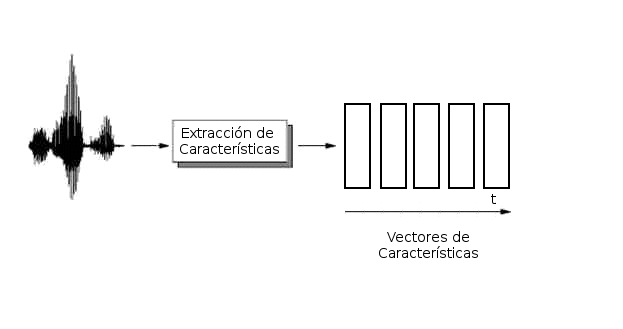
\includegraphics[width=0.8\textwidth]{./graphics/extraccion.png}
\caption{Fase de extracci\'on de caracter{\'\i}sticas. Gr\'afico basado en \cite{VerenichASR}.}
\label{figure:hmm}
\end{figure}
\end{frame}


\begin{frame}{Proceso B\'asico del Reconocimiento del Habla (6)}
\framesubtitle{Fase 2: Decodificaci\'on}
La fase de decodificaci\'on inicia con el conjunto de vectores de caracter{\'\i}sticas espectrales,
resultado de la fase de extracci\'on de caracter{\'\i}sticas.

El modelo de lenguaje busca predecir la probabilidad de una secuencia de palabras pertenecientes a un lenguaje.
Los modelos de lenguaje basados en n-gramas \cite{JelinekTheDevelopment1986} y los basados en 
gram\'aticas \cite{Wang2000} son com\'unmente utilizados.

\end{frame}

\begin{frame}{Proceso B\'asico del Reconocimiento del Habla (7)}
\framesubtitle{Fase 2: Decodificaci\'on}
El modelo ac\'ustico permite estimar la probabilidad de una entrada ac\'ustica dada una secuencia de palabras.
El mismo est\'a formado por varios HMM y el diccionario fon\'etico \cite{huang-handbook10}.

El algoritmo decodificador busca la secuencia de fonemas o subfonemas m\'as probable dados una 
secuencia de observaciones y un HMM. Este \'unico HMM se construye
mediante los componentes del modelo ac\'ustico y el modelo de lenguaje. El algoritmo de Viterbi y el 
algoritmo A* son dos algoritmos decodificadores utilizados frecuentemente en el reconocimiento del 
habla \cite{Jurafsky}.
\end{frame}

\begin{frame}{Proceso B\'asico del Reconocimiento del Habla (8)}
\framesubtitle{Fase 2: Decodificaci\'on}
La secuencia de fonemas o subfonemas puede convertirse a una secuencia de palabras utilizando el diccionario
fon\'etico que forma parte del modelo ac\'ustico.

Al finalizar la fase de decodificaci\'on se obtiene la secuencia de palabras m\'as probable dados los vectores
de caracter{\'\i}sticas espectrales, con lo cual llega a su culminaci\'on el proceso b\'asico
del reconocimiento del habla.

\begin{figure}[H] 
\centering
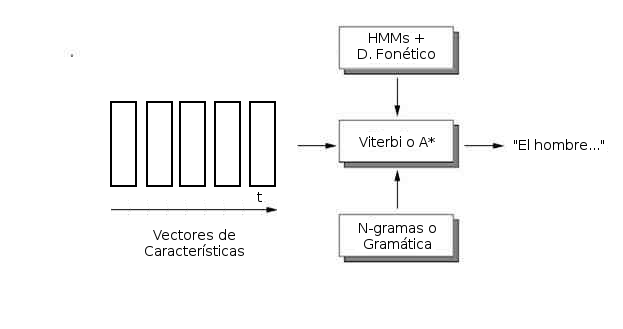
\includegraphics[width=0.8\textwidth]{./graphics/decodificacion.png}
\caption{Fase de decodificaci\'on. Gr\'afico basado en \cite{VerenichASR}.}
\label{figure:hmm}
\end{figure}
\end{frame}
